\chapter{Anhang}
\label{sec:Anhang}
\pagestyle{scrheadings}
EINFÜGEN:
Layout Stefan Erhard
Bilder Altium
3D Modelle
Dateien und Dateiverzeichnis (s. XMC Peripheral lib startseite)

\section{Seriennummern}
\label{app:Seriennummern}
Alle TDA5340 verfügen über eine eingebaute Seriennummer, welche ausgelesen werden kann. Die Seriennummern der verwendeten TDA5340 sind in der Tabelle aufgeführt.
\begin{table}[h]
\centering
\begin{tabular}{cc}
TDA & Seriennummer\\
\hline
TDA1 & 33020236\\
TDA2 & 11727080\\
TDA3& 11545236\\
TDA4& 11728870\\
TDA5& 11550773\\
TDA6& 33026263\\
\end{tabular}
\caption{Seriennummern der im Projekt verwendeten TDA5340 }
\label{default}
\end{table}

\section{3D-Daten}
\subsection{Gehäuse}
\label{app:Gehäuse}


\section{Layout TDA5340 Aufsteckboard}
Das Layout der Transceiver-Unterbaugruppen orientiert sich an dem Layout eines Aufsteckboards für den \enquote{XMC 2Go} damit ein TDA5340 auf mit diesem verwendet werden kann. 
\begin{figure}[tb]
\centering 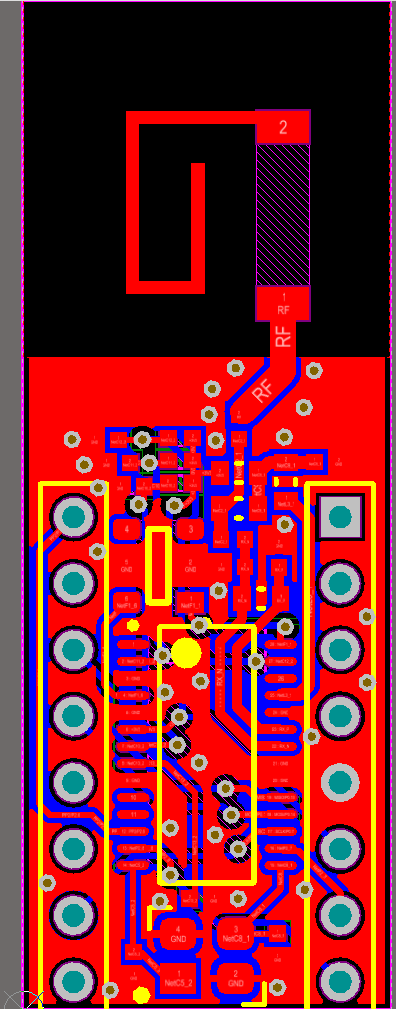
\includegraphics[width=5cm]{Abbildungen/Aufnahmen/Bilder/Altium/Layout Stefan Erhard/PCB Antenne.png} \caption{Ein Testbild mit einem Mandrill} \label{fig:testbild}
\end{figure}

test
\begin{figure}[htbp]
\begin{center}
\epsfile{file=Abbildungen/Aufnahmen/Bilder/Altium/Layout Stefan Erhard/PCB Antenne.png,scale=0.8}
\caption{{\bf default}}
\label{default}
\end{center}
\end{figure}



